\documentclass[aspectratio=169,10pt]{beamer}

% ---------------------------------------------------------------------------------------------
% Slides for a 10-minute talk. Build: latexmk -pdf slides.tex   (figures: ../report/figures/*.pdf)
% ---------------------------------------------------------------------------------------------
\usepackage[T1]{fontenc}
\usepackage{lmodern}
\usepackage{amsmath,amssymb}
\usepackage{booktabs}
\usepackage{graphicx}
\graphicspath{{../report/figures/}}

\definecolor{ink}{HTML}{0B0B0B}
\definecolor{ink2}{HTML}{52514E}
\definecolor{rhblue}{HTML}{2A78D6}
\definecolor{rhorange}{HTML}{EB6834}
\definecolor{rhgray}{HTML}{898781}
\definecolor{paper}{HTML}{FCFCFB}

\usetheme{default}
\usefonttheme{professionalfonts}
\setbeamertemplate{navigation symbols}{}
\setbeamercolor{background canvas}{bg=paper}
\setbeamercolor{normal text}{fg=ink}
\setbeamercolor{frametitle}{fg=ink}
\setbeamercolor{structure}{fg=rhblue}
\setbeamercolor{alerted text}{fg=rhorange}
\setbeamercolor{block title}{fg=ink,bg=rhblue!12}
\setbeamercolor{block body}{fg=ink,bg=rhblue!5}
\setbeamerfont{frametitle}{series=\bfseries,size=\Large}
\setbeamerfont{block title}{series=\bfseries,size=\normalsize}
\setbeamertemplate{itemize items}{\raisebox{0.15ex}{\small\textbullet}}
\setbeamertemplate{frametitle}{\vspace{0.45em}\insertframetitle\par\vspace{-0.3em}{\color{rhblue}\rule{2.2em}{1.2pt}}}
\setbeamertemplate{footline}{\hfill{\color{rhgray}\footnotesize\insertframenumber\,/\,\inserttotalframenumber}\hspace{1em}\vspace{0.6em}}
\setlength{\leftmargini}{1.2em}

\newcommand{\R}{\mathbb{R}}
\newcommand{\conv}{\operatorname{conv}}
\newcommand{\msum}{\oplus}
\newcommand{\cP}{\mathcal{P}}
\newcommand{\cE}{\mathcal{E}}
\newcommand{\LN}{\operatorname{LN}}
\newcommand{\src}[1]{{\color{rhgray}\footnotesize #1}}
\newcommand{\key}[1]{\textbf{\color{rhblue}#1}}

\title{Box or Simplex?}
\subtitle{A critical study of the Minkowski representation hypothesis}
\author{Omar Besbes}
\institute{Master MVA, ENS Paris-Saclay}
\date{}

\begin{document}

% ------------------------------------------------------------------------------------------ 1
\begin{frame}[plain]
  \vspace{2.2em}
  {\Huge\bfseries Box or Simplex?}\par\vspace{0.5em}
  {\Large A critical study of the Minkowski representation hypothesis}\par\vspace{0.3em}
  {\color{rhblue}\rule{3em}{1.5pt}}\par\vspace{1.3em}
  {\large Omar Besbes}\par
  {\color{ink2}Master MVA, ENS Paris-Saclay}\par\vspace{2.2em}
  \src{Project on: T.~Fel, B.~Wang et al., \emph{Into the Rabbit Hull: From Task-Relevant Concepts in DINO to Minkowski
  Geometry}, ICLR 2026.}
\end{frame}

% ------------------------------------------------------------------------------------------ 2
\begin{frame}{The paper in one slide}
  \begin{columns}[T,onlytextwidth]
    \column{0.47\textwidth}
    \textbf{Setting.} DINOv2 (ViT-B/14): an image becomes 261 tokens in $\R^{768}$.\par\medskip
    \textbf{Working assumption.} The linear representation hypothesis:
    \[ x=\sum_{j} z_j d_j,\quad z \text{ sparse},\quad \#\text{atoms}\gg 768 . \]
    \textbf{Tool.} A sparse autoencoder with 32,000 atoms.
    \column{0.49\textwidth}
    \begin{block}{Three parts}
      \begin{enumerate}
        \item \textbf{Tasks:} which atoms does a linear probe use?\\
        {\color{ink2}``Elsewhere'' concepts, borders, depth cues.}
        \item \textbf{Geometry:} is the dictionary what the hypothesis predicts?\\
        {\color{ink2}Dense, antipodal, clustered atoms: not quite.}
        \item \textbf{A new hypothesis:} tokens are sums of convex mixtures of archetypes.
      \end{enumerate}
    \end{block}
  \end{columns}
  \vfill
  \centering This talk is about the third part: \key{what does it assert, and what would contradict it?}
\end{frame}

% ------------------------------------------------------------------------------------------ 3
\begin{frame}{Two pictures of a representation}
  \begin{columns}[T,onlytextwidth]
    \column{0.47\textwidth}
    \begin{block}{Linear (LRH)}
      \[ x=\sum_{j\in S} z_j\,d_j,\qquad |S|\ \text{small} \]
      A concept is a \textbf{direction}.\\ More of it: a larger coefficient.\\ Activations: a union of cones.
    \end{block}
    \column{0.49\textwidth}
    \begin{block}{Minkowski (MRH)}
      \[ x=\sum_{i\in S} p_i,\qquad p_i\in\cP_i \]
      {\small $\cP_i$: convex hull of the archetypes of tile $i$.}\par\smallskip
      A concept is a \textbf{point or a region}.\\ More of it: closer to the archetype.\\
      Activations: sums of polytopes, $\cP_1\msum\cP_2\msum\cdots$
    \end{block}
  \end{columns}
  \bigskip
  \textbf{The paper's case.}
  \begin{itemize}
    \item Attention outputs convex combinations of values, and heads add up:
    $y=\sum_h W_O^{(h)}\sum_j \alpha_{h,j}v_{h,j}$.
    \item Three signatures: (E1) chords between tokens leave the data, (E2) archetypal analysis matches the
    autoencoder, (E3) co-activations of archetypes form blocks.
    \item Consequences: steering saturates; the decomposition is not identifiable from one layer.
  \end{itemize}
\end{frame}

% ------------------------------------------------------------------------------------------ 4
\begin{frame}{1. The two hypotheses are nested}
  \centering
  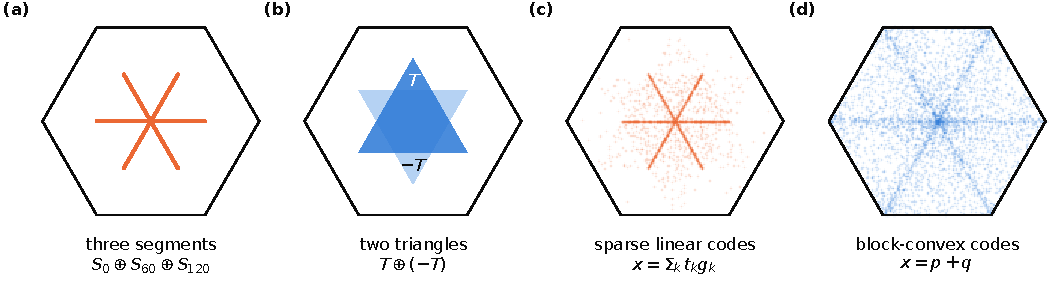
\includegraphics[width=0.93\textwidth]{fig_hexagon}
  \vspace{0.2em}
  \begin{columns}[T,onlytextwidth]
    \column{0.48\textwidth}
    \begin{itemize}
      \item A bounded linear feature is a tile with two archetypes: $z\,d=(1-\tfrac zM)\,0+\tfrac zM\,(Md)$.
      \item So \key{LRH $\subset$ MRH} (segments as tiles).
    \end{itemize}
    \column{0.48\textwidth}
    \begin{itemize}
      \item The only difference: codes of a group fill a \key{box} (independent) or a \key{simplex} (unit budget).
      \item The support cannot tell: the hexagon is both. The law of the codes can.
    \end{itemize}
  \end{columns}
\end{frame}

% ------------------------------------------------------------------------------------------ 5
\begin{frame}{2. What the attention argument shows}
  \begin{columns}[T,onlytextwidth]
    \column{0.52\textwidth}
    The statement is true for softmax, for \emph{any} weights:
    \begin{itemize}
      \item the values are the other tokens of the same image: the polytopes are \key{rebuilt for every image};
      \item it also holds for a random network;
      \item equality needs logits of rank $\ge 260$; a head has \key{rank 64};
      \item an update is not a token: within an image, \key{54\%} of the final token comes from MLPs.
    \end{itemize}
    \column{0.44\textwidth}
    \begin{block}{After the last LayerNorm: no polytope}
      Normalised tokens lie on an ellipsoid $\cE$.\par\smallskip
      $\cE$ contains no segment, so
      \begin{itemize}
        \item every chord between two tokens leaves $\cE$;
        \item a Minkowski sum inside $\cE$ is a single point.
      \end{itemize}
      \smallskip
      \src{Measured on DINOv2: $\|u\|/\sqrt d=1\pm10^{-7}$; midpoint of a chord at 10\% of the half-chord
      from $\cE$.}
    \end{block}
  \end{columns}
\end{frame}

% ------------------------------------------------------------------------------------------ 6
\begin{frame}{3. Signature E1: chords leave the sample, not the support}
  \centering
  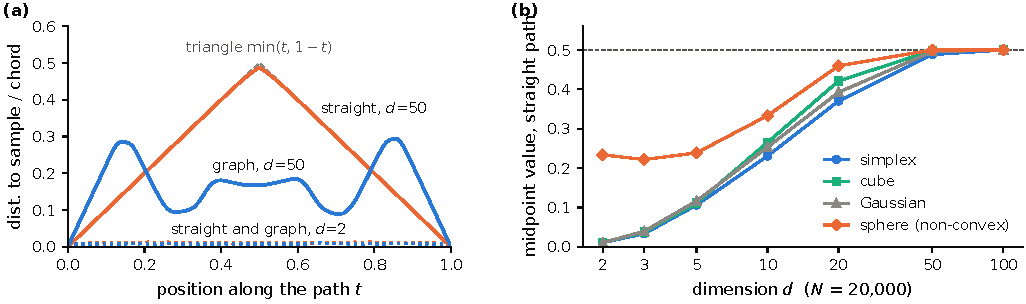
\includegraphics[width=\textwidth]{fig_chords}
  \vspace{0.1em}
  \begin{itemize}
    \item Uniform points in a \emph{convex} polytope: in high dimension the midpoint of a chord is far from every sample ($0.37$ of the chord at $d=20$, $0.49$ at $d=50$).
    \item DINOv2 tokens and a \key{Gaussian with the same covariance} give the same triangle ($0.50$); what differs is local density: the tokens are clustered.
  \end{itemize}
\end{frame}

% ------------------------------------------------------------------------------------------ 7
\begin{frame}{3. Signature E2: archetypal analysis in its sandwich}
  \begin{columns}[c,onlytextwidth]
    \column{0.43\textwidth}
    \centering
    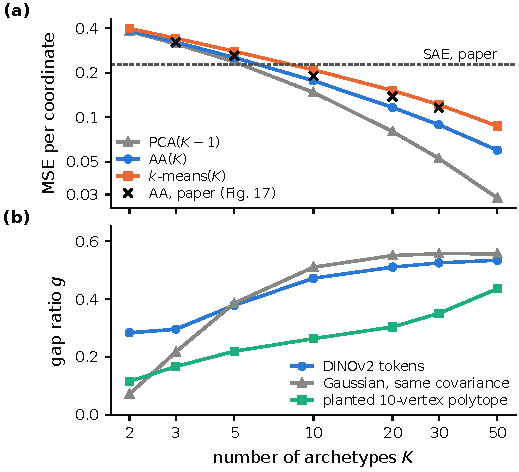
\includegraphics[width=\linewidth]{fig_sandwich}
    \column{0.53\textwidth}
    {\small\[ \mathrm{PCA}_{K-1}\le\mathrm{AA}_K\le k\text{-means}_K \]}
    \begin{itemize}
      \item We reproduce the paper's curve up to ten archetypes ($0.32$, $0.25$, $0.18$).
      \item With ten atoms per image, \key{$k$-means also beats the autoencoder} ($0.21<0.227$), and PCA does
      better still: the test rewards per-image models.
      \item Calibrated gap ratio at $K=10$: planted polytope $0.26$; Gaussian with the same covariance
      $0.51$; \key{DINOv2 tokens $0.47$}.
    \end{itemize}
  \end{columns}
\end{frame}

% ------------------------------------------------------------------------------------------ 8
\begin{frame}{3. Signature E3: a sum is not a union}
  \centering
  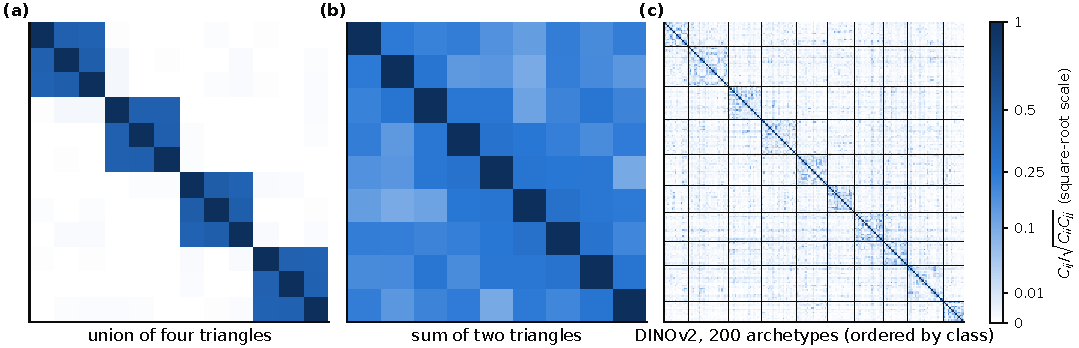
\includegraphics[width=0.9\textwidth]{fig_coactivation}
  \vspace{0.1em}
  \begin{itemize}
    \item Blocks mean that a token uses \emph{one} group of archetypes: a \key{union} of polytopes, i.e.\ clusters.
    \item A Minkowski \key{sum} activates all tiles together: archetypes are sums of vertices, co-activation is dense.
    \item On DINOv2 the blocks largely follow the image classes (adjusted mutual information $0.62$): one group per token, no sign of tiles adding up.
  \end{itemize}
\end{frame}

% ------------------------------------------------------------------------------------------ 9
\begin{frame}{4. Identifiability}
  \begin{columns}[T,onlytextwidth]
    \column{0.48\textwidth}
    \textbf{The paper:} a Minkowski sum does not determine its summands, so concepts cannot be recovered
    from one layer.
    \begin{itemize}
      \item Its proof subtracts a sublinear function from a support function; the difference need not be
      sublinear (a triangle has no segment as a summand).
      \item What is true: translations, splitting $\cP=\lambda\cP\msum(1-\lambda)\cP$, regrouping; and
      the hexagon $=$ three segments $=$ two triangles.
    \end{itemize}
    \column{0.48\textwidth}
    \textbf{What it does not show}
    \begin{itemize}
      \item It is a statement about \emph{supports} with \emph{all tiles active}.
      \item A support cannot tell a linear code from a block-convex one; within sums of segments, the
      generators are in fact determined.
      \item Dictionaries are identified by \key{sparsity and the law of the codes}; the hypothesis has both
      resources.
    \end{itemize}
  \end{columns}
\end{frame}

% ------------------------------------------------------------------------------------------ 9b
\begin{frame}{5. A factor we can observe: position}
  \begin{columns}[c,onlytextwidth]
    \column{0.5\textwidth}
    \centering
    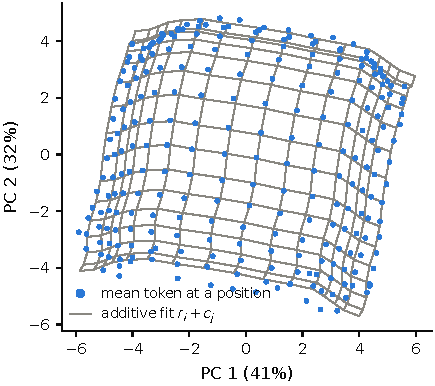
\includegraphics[width=0.95\linewidth]{fig_position}
    \column{0.46\textwidth}
    Mean token at position $(i,j)$ $\approx$ row effect $+$ column effect.
    \begin{itemize}
      \item $R^2=\key{0.974}$ ($0.947$ on held-out images, ceiling $0.952$): \key{a genuine Minkowski sum}.
      A positive result for the hypothesis.
      \item Each summand is an arc: $72$--$77\%$ of its variance on one direction, $96$--$97\%$ on two.
      A curve, not a simplex.
      \item Position is $4.8\%$ of the variance of the tokens.
      \item Always-on signed axes explain the dense and the antipodal atoms of the paper's dictionary.
    \end{itemize}
  \end{columns}
\end{frame}

% ------------------------------------------------------------------------------------------ 10
\begin{frame}{Conclusion}
  \begin{columns}[T,onlytextwidth]
    \column{0.48\textwidth}
    \textbf{What stands}
    \begin{itemize}
      \item Parts I and II: a sparse, non-negative, nearly orthogonal code is too narrow for DINOv2.
      \item The hypothesis asks a real question: do features \emph{compete} inside groups?
      \item Additive composition holds where we can test it (position, $97\%$).
    \end{itemize}
    \smallskip
    \textbf{What does not follow}
    \begin{itemize}
      \item The three signatures: passed by data without archetypes.
      \item Exact Minkowski geometry after LayerNorm.
      \item Non-identifiability as a special feature of the hypothesis.
    \end{itemize}
    \column{0.48\textwidth}
    \textbf{What would count as evidence}
    \begin{itemize}
      \item Joint statistics of the codes of a group: \key{box or simplex?} On factors of known value.
      \item Before the last normalisation, or along the ellipsoid.
      \item Per head, with the attention weights as codes.
    \end{itemize}
    \smallskip
    \textbf{Limits of this study}
    \begin{itemize}
      \item One model, 1,000 images, nulls matched to second moments, no access to the paper's dictionary.
    \end{itemize}
  \end{columns}
\end{frame}

% ------------------------------------------------------------------------------------------ backup
\appendix
\begin{frame}{Backup: the three signatures at a glance}
  \centering\footnotesize
  \begin{tabular}{@{}lccc@{}}
    \toprule
    & DINOv2 tokens & Null (no archetypes) & Planted structure\\
    \midrule
    (E1) midpoint dist.\ / chord & $0.50$ (graph $0.16$) & Gaussian: $0.50$ ($0.19$) & simplex: $0.49$ ($0.15$)\\
    (E2) gap ratio at $K=10$ & $0.47$ & Gaussian: $0.51$ & polytope: $0.26$\\
    (E3) co-activation & blocks = classes & union: $99.9\%$ in blocks & sum: no blocks\\
    \bottomrule
  \end{tabular}
  \bigskip

  \raggedright
  \textbf{Data.} Patch tokens of 1,000 Imagenette images, last layer of DINOv2 ViT-B/14 with registers, after the
  final normalisation; $50{,}000$ tokens for (E1), 200 images for (E2), 100 images and 200 archetypes for (E3).
\end{frame}

\begin{frame}{Backup: no segment after layer normalisation}
  $\LN(x)=\gamma\odot u+\beta$ with $u=\dfrac{x-\mu(x)\mathbf 1}{\sigma(x)}$, so $\mathbf 1^\top u=0$ and $\|u\|^2=d$:
  $u$ lies on a sphere $\mathbb S$.\par\medskip
  \begin{itemize}
    \item If $u\neq u'$ on $\mathbb S$ and $0<s<1$, then $\|(1-s)u+su'\|<\sqrt d$ (strict convexity of the norm).
    \item $u\mapsto\gamma\odot u+\beta$ is affine and injective ($\gamma_k\neq0$): segments go to segments, and the
    image $\cE$ of $\mathbb S$ contains none.
    \item If $\cP_1\msum\dots\msum\cP_m\subseteq\cE$ and some $\cP_i\ni p\neq p'$, then $q+[p,p']\subseteq\cE$:
    contradiction.
  \end{itemize}
  \medskip
  \textbf{On DINOv2:} $0.19\le\gamma_k\le 14.9$; tokens of one image are $56^\circ$ apart on average; the midpoint of
  their chord is at $10\%$ of the half-chord from $\cE$.
\end{frame}

\begin{frame}{Backup: the gap in the non-identifiability proof}
  Support function: $h_C(u)=\sup_{x\in C}\langle u,x\rangle$, and $h_{A\msum B}=h_A+h_B$.\par\medskip
  The proof takes any sublinear $s$ with $0\le s\le h_X$ and writes $h_X=(h_X-s)+s$.\par\medskip
  \textbf{Counter-example.} $X$ = unit equilateral triangle centred at $0$, $Q=[-0.1,0.1]\times\{0\}$, $s=h_Q$.
  \begin{itemize}
    \item $0\le s\le h_X$ in every direction.
    \item $f=h_X-s$: $f(u)=f(v)=0.45$ for $u,v$ at $60^\circ$ and $120^\circ$, but $f(u+v)=1>0.9$.
    \item So $f$ is not subadditive: $Q$ is not a summand of a triangle.
  \end{itemize}
  \medskip
  What is true: translations, $\cP=\lambda\cP\msum(1-\lambda)\cP$, regrouping; and
  hexagon $=$ three segments $=$ triangle $\msum$ reflected triangle.
\end{frame}

\end{document}
